\section{Questões}

\begin{enumerate}
 \item (VUNESP - 2017) Uma sorveteria vende os sorvetes em copinhos pequenos, médios ou grandes, cuja soma dos respectivos preços unitários é igual a $R\$ 42,00$. Sabe-se que os preços unitários dos copinhos médio e grande correspondem, respectivamente, a $\frac{7}{4}$ e $\frac{5}{2}$ do preço do copinho pequeno. Desse modo, é correto afirmar que cada copinho grande é vendido por
 \begin{multicols}{5}
 \begin{enumerate}[a)]
 \item $R\$ 16,00$
 \item $R\$ 16,50$
 \item $R\$ 18,50$
 \item $R\$ 20,00$
 \item $R\$ 21,00$
 \end{enumerate}
 \end{multicols}

 \item (IBFC - 2017) Alípio foi ao hortifruti e comprou laranjas e limões, no total de $22$ unidades. O número de laranjas é igual ao número de limões diminuído de $6$ unidades. Desse modo, o número de limões comprados por Alípio foi:
 \begin{multicols}{5}
 \begin{enumerate}[a)]
 \item $8$
 \item $10$
 \item $14$
 \item $16$
 \item $17$
 \end{enumerate}
 \end{multicols}

 \item (UVA - 2016) Dois amigos praticam um jogo mental usando números decimais. José diz um número natural qualquer e Tiago deve multiplicá-lo por $0,6$, depois somar $3,2$ e, por fim, dividir este resultado por $0,5$. Se Tiago obteve $12,4$, então o número dito por José foi:
 \begin{multicols}{5}
 \begin{enumerate}[a)]
 \item $4$
 \item $5$
 \item $6$
 \item $7$
 \end{enumerate}
 \end{multicols}

 \item (NC-UFPR - 2017) Considere a equação dada por $2x^2 + 12x + 3 = -7$. Assinale a alternativa que apresenta a soma das duas soluções dessa equação.
 \begin{multicols}{5}
 \begin{enumerate}[a)]
 \item $0$
 \item $1$
 \item $-1$
 \item $6$
 \item $-6$
 \end{enumerate}
 \end{multicols}

 \item (UEM - 2017) Se $m$ e $n$ são as soluções da equação  $2x^2 +9x - 5 = 0$  e $m$ é maior do que $n$, então o valor de $n +10m$ é igual a
 \begin{multicols}{5}
 \begin{enumerate}[a)]
 \item $0$
 \item $5$
 \item $-5$
 \item $10$
 \item $-10$
 \end{enumerate}
 \end{multicols}

 \item (PUC-PR - 2017) A equação $8x^2 – 28x + 12 = 0$ possui raízes iguais a $x_1$ e $x_2$. Qual o valor do produto $x_1 \cdot x_2$?
 \begin{multicols}{5}
 \begin{enumerate}[a)]
 \item $\frac{1}{2}$
 \item $3$
 \item $\frac{3}{2}$
 \item $12$
 \item $28$
 \end{enumerate}
 \end{multicols}

 \item (IBFC - 2017) A alternativa que apresenta a equação de 2.º grau cujas raízes reais são $5$ e $(-1)$ é:
 \begin{enumerate}[a)]
 \item $x^2 + 4x + 5 = 0$
 \item $x^2 + 4x^2 – 5 = 0$
 \item $2x^2 - 2x + 10 = 0$
 \item $2x^2 + 2x – 10 = 0$
 \item $x^2 - 4x – 5 = 0$
 \end{enumerate}

 \item (UNISUL - 2016) Considere as proposições:
 \begin{enumerate}[I)]
 \item O valor de $350^2 - 349^2 = 1$.
 \item O valor numérico da expressão  $x^2+ 2x + 1 / x+1$ quando $x = 1523$ é $1524$.
 \item A igualdade $4x^2 - 36 / 2x + 6 = 2x - 6$ , para todo $x \in \R$.
 \item $(√3 + 5)2 = (√3)2 + 52 = 3 + 25 =28$.
 \end{enumerate}
 É(são) verdadeira(s) a(s) proposição(ões):
 \begin{enumerate}[a)]
 \item I, II e IV.
 \item Apenas a I.
 \item Apenas a III.
 \item II e III.
 \item Apenas a II.
 \end{enumerate}

 \item (UNISUL - 2016) Sejam $r$ e $s$ as raízes da equação $x^2 - 9x + 13 = 0$, assinale a alternativa que corresponde ao valor numérico da expressão $(r + s)^2 + 4rs$.
 \begin{multicols}{5}
 \begin{enumerate}[a)]
 \item 131.
 \item 129.
 \item 130.
 \item 133.
 \item 132.
 \end{enumerate}
 \end{multicols}

 \item (COPESE-UFPI - 2016) Djair está casado há $m$ anos. Se ele permanecer casado por mais $30$ anos, ele irá estar casado por $m^2$ anos. Pode-se afirmar que Djair já está casado há:
 \begin{multicols}{5}
 \begin{enumerate}[a)]
 \item 3 anos.
 \item 4 anos.
 \item 5 anos.
 \item 6 anos.
 \item 7 anos.
 \end{enumerate}
 \end{multicols}

 \item (Sociesc - 2010) Em uma cidade existem duas locadoras de automóveis. A locadora A cobra uma taxa fixa de R\$ 50,00 por dia e R\$ 1,50 por quilômetro rodado. A locadora B cobra uma taxa fixa de R\$ 30,00 por dia e R\$ 2,00 por quilômetro rodado. Sendo assim, podemos afirmar que, em um dia:
  \begin{enumerate}
  \item A locadora B é mais vantajosa somente para um percurso superior a 40 quilômetros.
  \item Para qualquer quilometragem é sempre vantagem usar a locadora A.
  \item Para qualquer quilometragem é sempre vantagem usar a locadora B.
  \item O preço é o mesmo nas duas locadoras independente da quilometragem.
  \item A locadora A é mais vantajosa somente para um percurso superior a 40 quilômetros.
 \end{enumerate}

\item (Sociesc - 2009) Quando $\sqrt{x + \sqrt{2x+3}}= \sqrt{4x-6}$ o valor de $-x^2+1$ é:
 \begin{enumerate}
  \item 10
  \item $\frac{11}{9}$
  \item $\pm 1$
  \item -8
 \end{enumerate}

 \item (Sociesc - 2009) Na equação $ax^2+bx+c-k=0$ tem-se os seguintes valores para o par $(x, k): (0,-1), (2,-1) \text{ e } (-1,-4)$. Nessas condições, a(s) raízes da equação quando $k=0$ podem ser expressa(s) como:
 \begin{enumerate}
  \item $\pm 1$
  \item 1
  \item -1
  \item 0
 \end{enumerate}

 \item (Sociesc - 2009) João perguntou à sua irmã quantos metros de fita dupla face deveria comprar, para prender uma toalha em uma mesa retangular, na festa de rua que estavam organizando. Sua irmã deu-lhe a seguinte resposta: a mesa retangular tem 3 metros a mais de comprimento que a largura. Como a área da mesa é $10 m^2$, concluímos que seu perímetro é:
  \begin{enumerate}
  \item 14 metros
  \item 15 metros
  \item 13 metros
  \item 16 metros
 \end{enumerate}

 \item (Sociesc - 2009) Existem dois números, $x_1$ e $x_2$ , que satisfazem a seguinte condição: "o seu quadrado é igual ao seu triplo”. A soma de $x_1$ e $x_2$ é:
  \begin{enumerate}
  \item 5
  \item 2
  \item 4
  \item 3
 \end{enumerate}

 \item (Sociesc - 2010) A soma das raízes das equações $\frac{x}{6}+\frac{x}{3}=18$ e $4x^2-64=0$ é igual a:
  \begin{enumerate}
  \item 40
  \item -36
  \item 44
  \item -44
  \item 36
 \end{enumerate}

  \item (Sociesc - 2010) Pense em um número, disse João a Pedro, e faça o que eu pedir, pois vou adivinhar o resultado das operações matemáticas feitas com o número que você pensou. Pedro pensou num número e João começou a dizer as operações que ele deveria fazer: calcule o dobro do número que você pensou e some 7 unidades; multiplique este resultado por 4, subtraia 28 e divida o resultado pelo próprio número. Após Pedro ter feito os cálculos, João olhou para ele e “adivinhou” que o resultado era:
  \begin{enumerate}
  \item 8
  \item -8
  \item 4
  \item -4
  \item 10
 \end{enumerate}

 \item (Sociesc - 2010) O ponto do eixo das \sout{abscissas} (ordenadas) equidistante dos pontos $A(-1, 1)$ e $B(3, 2)$ é:


 \begin{multicols}{2}

 \begin{enumerate}
  \item $(0, \frac{15}{2})$
  \item $(0, \frac{9}{2})$
  \item $(0,5)$
  \item $(0, \frac{17}{2})$
  \item $(0, \frac{11}{2})$
 \end{enumerate}

 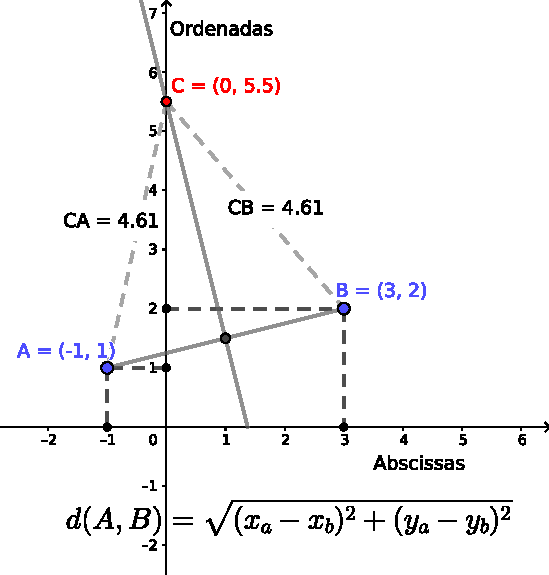
\includegraphics[width=5cm]{../Capitulos/Figuras/dist_exer1.pdf}

 \end{multicols}

 \item (Sociesc - 2009) Um fazendeiro dividirá seu terreno em três partes para plantar milho, soja e trigo. A área onde será plantado o milho terá o dobro da área onde será plantada a soja, que por sua vez terá o dobro da área do trigo. O terreno tem área de 42 hectares. As áreas reservadas para a plantação do milho, da soja e do trigo, serão, respectivamente:
  \begin{enumerate}
  \item 12, 24 e 6 hectares
  \item 20, 10 e 2 hectares
  \item 14, 14 e 14 hectares
  \item 24, 12 e 6 hectares
 \end{enumerate}

 \item (SOCIESC - Téc. Enfermagem) Na prova da matéria X, o professor decidiu colocar 20 questões, das quais cada certa vale 1 ponto e cada errada decresce 0,5 pontos. Assim, uma pessoa que acertou 12 questões obteve a nota:
  \begin{enumerate}
  \item Mínima
  \item Maior do que 7
  \item Maior do que 10
  \item Menor do que 7
  \item Máxima
 \end{enumerate}

 \item (SOCIESC - Téc. Enfermagem) O valor de $x$ em: $4x-7=2(3x-8)$ é:
 \begin{enumerate}
  \item 4,5
  \item 18
  \item 0,5
  \item 0,3
  \item 2
 \end{enumerate}

 \item (Lógica - Fundatec - 2018) Uma locadora de máquinas de café expresso cobra uma taxa diária de R\$ 83,00 e R\$ 0,30 por café de 50ml produzido. Quanto pagaria a organização de um evento na locação de um máquina durante 5 dias se produzisse 400 cafés expressos de 50ml?
\begin{multicols}{2}
\begin{enumerate}[a)]
\item 490,00
\item 535,00
\item 1.615,00
\item 6.000,00
\item 6.415,00
\end{enumerate}
\end{multicols}

 \item (UDESC/IBC - 2009) Se $x$ e $y$ são números reais tais que $2x + y = 8$, o valor máximo do produto $x \cdot y$ é:
 \begin{enumerate}
 \item 24
 \item 20
 \item 16
 \item 12
 \item 8
 \end{enumerate}

 \item (UDESC/IBC - 2009) Para que valores de $m$ a equação $4x^2- 4mx + (4m – 3) = 0$ não admite raízes reais?
 \begin{enumerate}
 \item $\{m \in \R \mid 1< m < 3\}$
 \item $\{\forall m \mid m \in \R\}$
 \item $\{m \in \R \mid m < 1 \text{ ou } m > 3\}$
 \item $m > 0$
 \item nenhum valor real de $m$.
 \end{enumerate}

 \item (TJ/SC - 2018) Em uma fila há 70 pessoas, entre as quais Pedro e João. Sabe-se que:
  \begin{itemize}
   \item Pedro está na frente de João e há duas pessoas entre eles;
   \item O número de pessoas na frente de Pedro é o dobro do número de pessoas atrás de João.
  \end{itemize}
  Nessa fila João ocupa o:
  \begin{enumerate}
  \item 45ª lugar
  \item 46ª lugar
  \item 47ª lugar
  \item 48ª lugar (*)
  \item 49ª lugar
 \end{enumerate}

 \end{enumerate}

 Gabarito: 1 d); 2 c); 3 b); 4 e); 5 a); 6 c); 7 e); 8 d); 9 d); 10 d); 11 e); 12 d); 13 b); 14 a); 15 d); 16 e); 17 a); 18 e); 19 d); 20 b); 21 a); 22 b); 23 e); 24 a).
